%Thanks to Prof. Bazioch for the use of his template
%TeXMaker on a PC or Linux and TeXShop on a mac are good editors for
%creating LaTeX documents
%A good place to get started with LaTeX is
%http://ctan.mirrors.hoobly.com/info/Math_into_LaTeX-4/Short_Course.pdf
\documentclass[12pt]{article}
\usepackage{amsmath,amssymb,amsthm}
\usepackage{graphicx}
\usepackage{caption}
\usepackage{subcaption}


\usepackage{enumerate,multicol,verbatim}
\usepackage{fullpage}

\setlength{\parindent}{0in}
\setlength{\parskip}{3mm}
\newcommand{\nline}{\rule{\linewidth}{0.5pt}}

\theoremstyle{plain}
\newtheorem{theorem}{Theorem}
\newtheorem{lemma}[theorem]{Lemma}
\newtheorem{proposition}[theorem]{Proposition}
\newtheorem{corollary}[theorem]{Corollary}

\theoremstyle{definition}
\newtheorem{definition}[theorem]{Definition}
\newtheorem{notation}[theorem]{Notation}
\newtheorem{remark}[theorem]{Remark}
\newtheorem{note}[theorem]{Note}
\newtheorem{nn}[theorem]{}



% document title YOU DO NOT NEED TO CHANGE THIS
\makeatletter
\renewcommand{\maketitle}{
\begin{center}
\nline\\
\vspace{2ex}
{\huge \textsc{\@title}}
\nline\\
{\large\textsc{\@author \hfill \@date}}
\vspace{4ex}
\end{center}
}
\makeatother
%%%

%%%%%%%%%%%%%%%%%%%%%%%%%%%%%%%
%%%%%%%%%%%%%%%%%%%%%%%%%%%%%%%

%%%%%%% THIS SHOULD BE CHANGED FOR EACH NEW ASSIGNMENT

\title{HPC I Homework 1}

%%%%%%% BE SURE TO PUT IN YOUR OWN NAME

\author{Morse, Michael}

%%%%%%% BE SURE TO PUT IN THE DUE DATE

\date{October 5, 2017}

%%%%%%%%%%%%%%%%%%%%%%%%%%%%%%%
%%%%%%%%%%%%%%%%%%%%%%%%%%%%%%%


\begin{document}

\maketitle
\newpage
%%%%%%%%%%%%%%%%%%%%%%%%%%%%%%%
%Problem 1
%%%%%%%%%%%%%%%%%%%%%%%%%%%%%%%

\section*{Problem 1}
My error check code is in the hw2 folder and is called by all codes in this assignment. For the error check code I had the error code looked up, printed to screen than I called MPI\_ABORT. Therefore, the difference between my error handling the default is that mine will print look up the error code by then abort.
\section*{Problem 2}
For the ping-pong problem I sent INTEGER(kind=8) 8 byte FORTRAN integers back and forth between two processors and had processor 0 time how long it took. I did this for array sizes 1 (8 byte) to one million (1 Mbyte). I did this in step size of 100 bytes. Unfortunately this resulted in a lot of noise in my plots. The latency is plotted vs message size where latency is half the time it took for the message to send and receive. I also plotted the bandwidth vs message size where bandwidth is calculated as message size over latency.  

We can estimate a bandwidth of about 1500 Mbytes/second and a latency on the order of millisecond for a latency.
\begin{figure*}[t]
    \centering
    \begin{subfigure}[t]{0.5\textwidth}
        \centering
        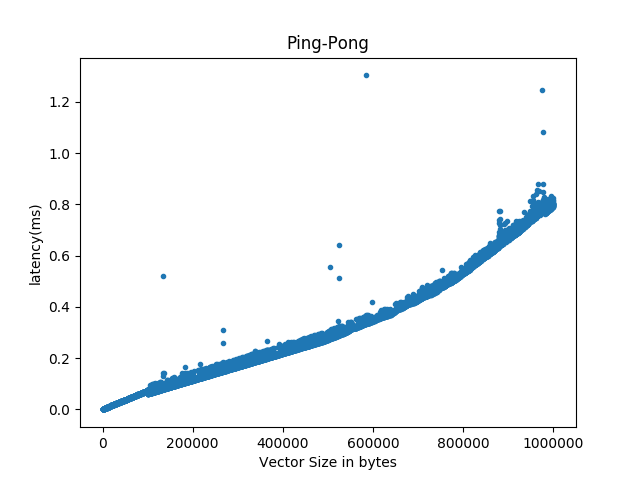
\includegraphics[height=2.2in]{latency.png}
        \caption{latency vs message size for ping pong}
    \end{subfigure}%
    ~
    \begin{subfigure}[t]{0.5\textwidth}
        \centering
        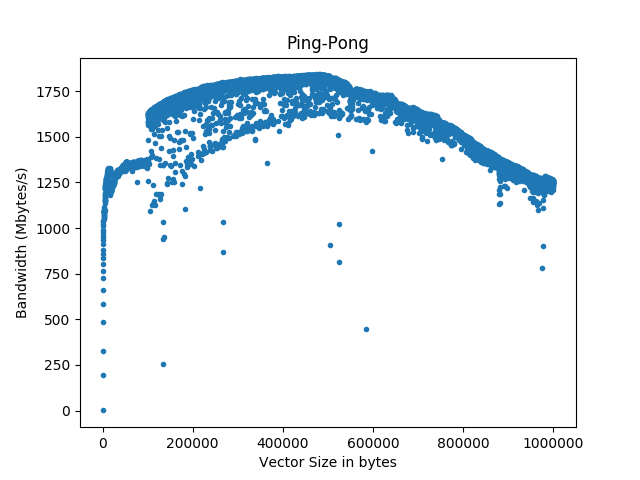
\includegraphics[height=2.2in]{bandwidth.png}
        \caption{Bandwidth vs message size for ping pong}
    \end{subfigure}
\end{figure*}



\section*{Problem 3}

\subsection*{Serial}


We see that as the grid size increases the area gets better until a grid of about 1000 by 1000 where is begins to level off.

\begin{figure*}[t!]
    \centering
    \begin{subfigure}[t]{0.5\textwidth}
        \centering
        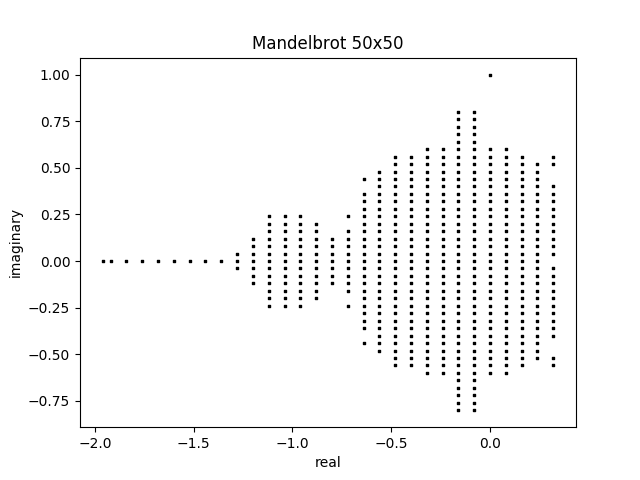
\includegraphics[height=1.2in]{mandelbrot_course_a.png}
        \caption{Course Mandelbrot set}
    \end{subfigure}%
    ~
    \begin{subfigure}[t]{0.5\textwidth}
        \centering
        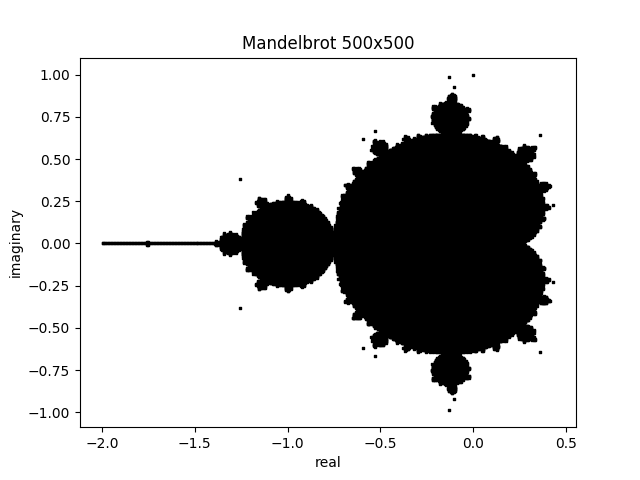
\includegraphics[height=1.2in]{mandelbrot_medium_a.png}
        \caption{Medium Mandelbrot set}
    \end{subfigure}
    ~
        \begin{subfigure}[t]{0.5\textwidth}
        \centering
        
\includegraphics[height=1.2in]{mandelbrot_fine_a.png}
        \caption{Fine Mandelbrot set}
    \end{subfigure}%
    \caption{Serial Mandelbrot sets for serial}
\end{figure*}
\begin{figure*}
 \centering
        
\includegraphics[width=0.5\textwidth]{area_a.png}
        \caption{area vs grid size for serial }
\end{figure*}


\subsection*{MPI-row by row}

For the first way of running the code in parallel I elected to send each processor a the a box with height 2 and width depending on the number of processors. As the load was not balanced in the case some processors were working harder then others. For example the ones at the end had very little work as the Mandelbrot set does not extend to $x=2$.

As for area vs grid size we see the same trend as before, the area only gets marginally better after a grid size of about 1000.

As for time vs number of course, how the code was written each core was splitting their grid into $nxn$ points so increasing the number of cores increased the accuracy of the area and point density but did not decrease the time. Instead it increased the time with the number of cores as the cores in heavy dense areas had much more work to do. A time saving approach would have been to take the grid and divide by number of cores squared so it scaled. I think this would have a decrease time with increased cores.
\begin{figure*}[t!]
    \centering
    \begin{subfigure}[t]{0.5\textwidth}
        \centering
        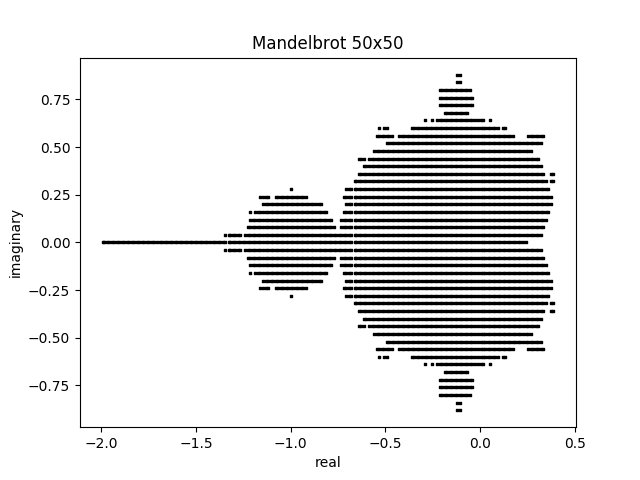
\includegraphics[height=1.2in]{mandelbrot_course_b.png}
        \caption{Course Mandelbrot set}
    \end{subfigure}%
    ~
    \begin{subfigure}[t]{0.5\textwidth}
        \centering
        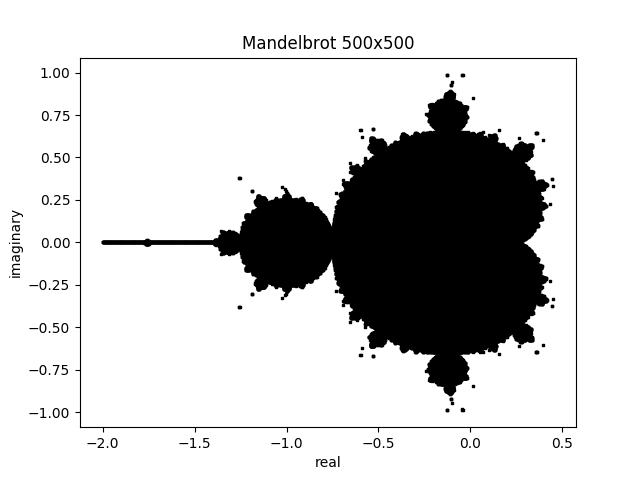
\includegraphics[height=1.2in]{mandelbrot_medium_b.png}
        \caption{Medium Mandelbrot set}
    \end{subfigure}
    ~
        \begin{subfigure}[t]{0.5\textwidth}
        \centering
        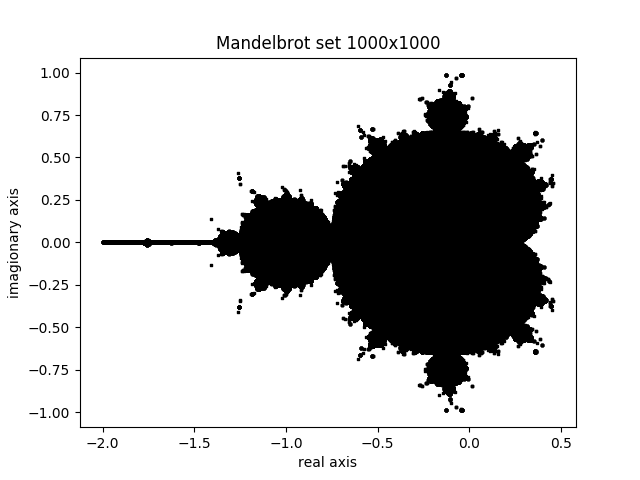
\includegraphics[height=1.2in]{mandelbrot_fine_b.png}
        \caption{Fine Mandelbrot set}
    \end{subfigure}%
    \caption{Row By Row Mandelbrot sets}
\end{figure*}

\begin{figure*}
 \centering
        
\includegraphics[width=0.5\textwidth]{time_b.png}
        \caption{time vs number of cores for row by row}
\end{figure*}
\begin{figure*}
 \centering
        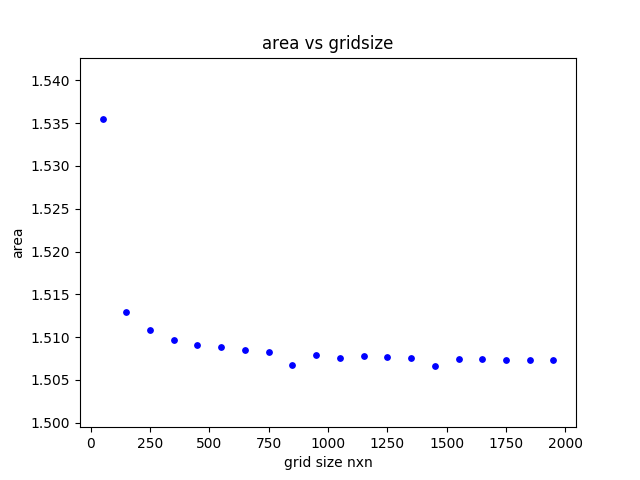
\includegraphics[width=0.5\textwidth]{area_b.png}
        \caption{area vs grid size for row by row}
\end{figure*}



\subsection*{MPI-round robin} 

For the round robin approach I made rank 0 the master. Each slave would send a non-blocking request to let the master know it was ready for a new point. The master would distribute the work point wise instead of grid wise. This evenly distributed the work over all processors so the point density in any one sub grid did not matter.

Here we have the same observation for area but as the work is being evenly distributed across all cores we also see that in increases the speed. From 4 cores to 8 cores we about half the time it takes, and by the time we are at 16 cores the time is about 30\% of what it was at 4.

\begin{figure*}[t!]
    \centering
    \begin{subfigure}[t]{0.5\textwidth}
        \centering
        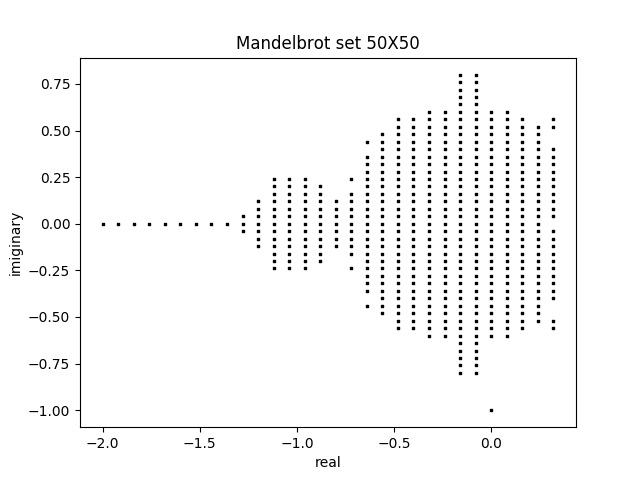
\includegraphics[height=1.2in]{mandelbrot_course_c.png}
        \caption{Course Mandelbrot set}
    \end{subfigure}%
    ~
    \begin{subfigure}[t]{0.5\textwidth}
        \centering
        
\includegraphics[height=1.2in]{mandelbrot_medium_c.png}
        \caption{Medium Mandelbrot set}
    \end{subfigure}
    ~
        \begin{subfigure}[t]{0.5\textwidth}
        \centering
        
\includegraphics[height=1.2in]{mandelbrot_fine_c.png}
        \caption{Fine Mandelbrot set}
    \end{subfigure}%
    \caption{Round Robin Mandelbrot sets}
\end{figure*}

\begin{figure*}
 \centering
        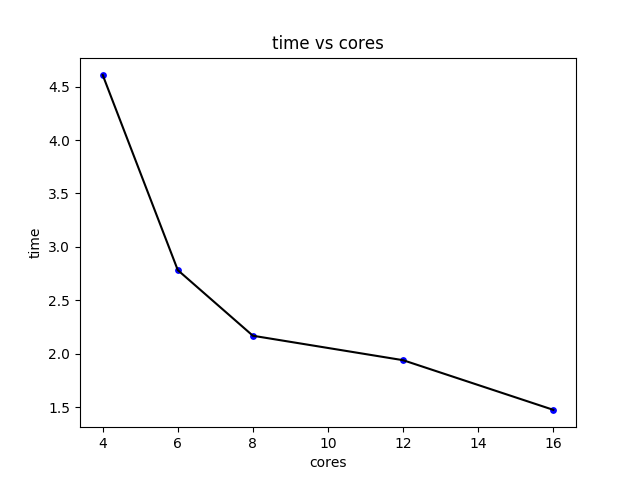
\includegraphics[width=0.5\textwidth]{time_c.png}
        \caption{time vs number of cores for round robin}
\end{figure*}

\begin{figure*}
 \centering
        
\includegraphics[width=0.5\textwidth]{area_c.png}
        \caption{area vs grid size for round robin}
\end{figure*}

\end{document}
